\documentclass[12pt, a4paper]{article}

\usepackage{ctex}
\usepackage{float, booktabs, parskip, enumerate, pythonhighlight}
\usepackage{amsmath, amsthm, amssymb, mathrsfs, bm}
\usepackage{graphicx, subfigure, svg}
\usepackage{hyperref, endnotes}

\setlength{\parindent}{4em}
\setlength{\parskip}{1em}
\allowdisplaybreaks[4]

\newcommand{\ivec}{\bm}

\newcommand{\NN}{\mathcal{N}}
\newcommand{\al}{\overline{\alpha}}


\title{{\Huge{\textbf{Report on Homework 3 \\}}} —— Deep Learning}
\author{刘滨瑞 \\ 2021012579 \quad 未央-水木12}

\begin{document}

\maketitle

\section{Transformer}

    运行环境为：Ubuntu 22.04.3 LTS，Python 3.9.18，PyTorch 2.1.2。

    \subsection{Task1: Standard Transformer Model}

        参考原论文和课件中给出的相关公式，我们补全了标准的Transformer模型，
        源代码参见./Transformer/layers/attention.py中的MultiHeadAttention类和multi\_head\_attention函数。 \endnote{Vaswani, A., Shazeer, N., Parmar, N., Uszkoreit, J., Jones, L., Gomez, A. N., Kaiser, L., \& Polosukhin, I. (2017). Attention is all you need. In I. Guyon, U. V. Luxburg, S. Bengio, H. Wallach, R. Fergus, S. Vishwanathan, \& R. Garnett (Eds.), Advances in Neural Information Processing Systems 30 (pp. 5998–6008).}

        训练过程中，模型在验证集、测试集和训练集上的loss变化曲线如图1所示。
        可以看出，模型收敛较快，6个epochs时模型在验证集上的loss已不再继续降低。

        \begin{figure}[htbp]
        \centering
        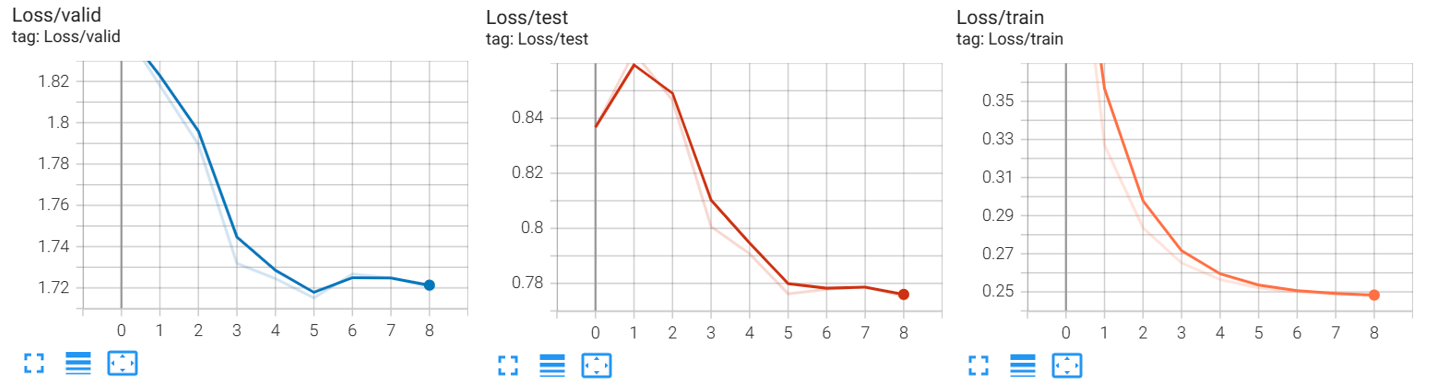
\includegraphics[width=1\textwidth]{./assets/Transformer/curve.png}
        \caption{模型在验证集、测试集和训练集上的loss变化曲线}
        \end{figure}

        \begin{figure}[htbp]
        \centering
        \subfigure[id = 0]{
\includegraphics[width=0.48\columnwidth]{./assets/Transformer/0.pdf}}
        \subfigure[id = 20]{
\includegraphics[width=0.48\columnwidth]{./assets/Transformer/20.pdf}}
        \subfigure[id = 40]{
\includegraphics[width=0.48\columnwidth]{./assets/Transformer/40.pdf}}
        \subfigure[id = 60]{
\includegraphics[width=0.48\columnwidth]{./assets/Transformer/60.pdf}}
        \caption{标准模型的部分预测结果}
        \end{figure}

        如图2所示，我们展示了部分的预测结果，发现模型进行回归预测的效果并不是特别理想。
        推测可能的原因有两点。
        一是数据量较少，特征与预测值间的相关性不高，因此回归预测任务的难度较大；
        二是在我们使用的Transformer模型中，层数、注意力头数，隐藏层参数量都很少，模型的拟合能力有限。

        取在验证集上表现最好的模型，在测试集上计算误差，结果为：
        \begin{itemize}
            \item MSE: 0.775672197341919
            \item MAE: 0.648556411266327
        \end{itemize}

    \subsection{Task2: Technical Details}

        在回归预测任务中，为保证模型是自回归的，我们在训练过程中会在预测值及其之后的内容上添加mask，
        以此来强制要求模型在学习时只能看到预测值之前的内容。
        否则，模型在训练时可能会“作弊”，即错误地使用了在推理过程本不可见的未来信息，
        最终导致模型无法学习到某些可泛化的数据规律。

        实现mask的方法很简单，只需要在计算注意力时，
        在softmax算子前将attention张量中预测值及其之后内容的相应位置上的值设置为-inf即可（在本例中即为矩阵的上三角部分）。
        代码实现如下：

\begin{python}
if attn_mask is not None:
    attn = attn.masked_fill(th.logical_not(attn_mask), -th.inf)
attn = nn.functional.softmax(attn, dim=3)
\end{python}

    \subsection{Task3: Attention Visualization}

        在Transformer模型中，我们截取出最后一层Encoder的attention值，
        将其可视化为热力图的形式，结果如图3所示。

        \begin{figure}[htbp]
        \centering
        \subfigure[id = 0]{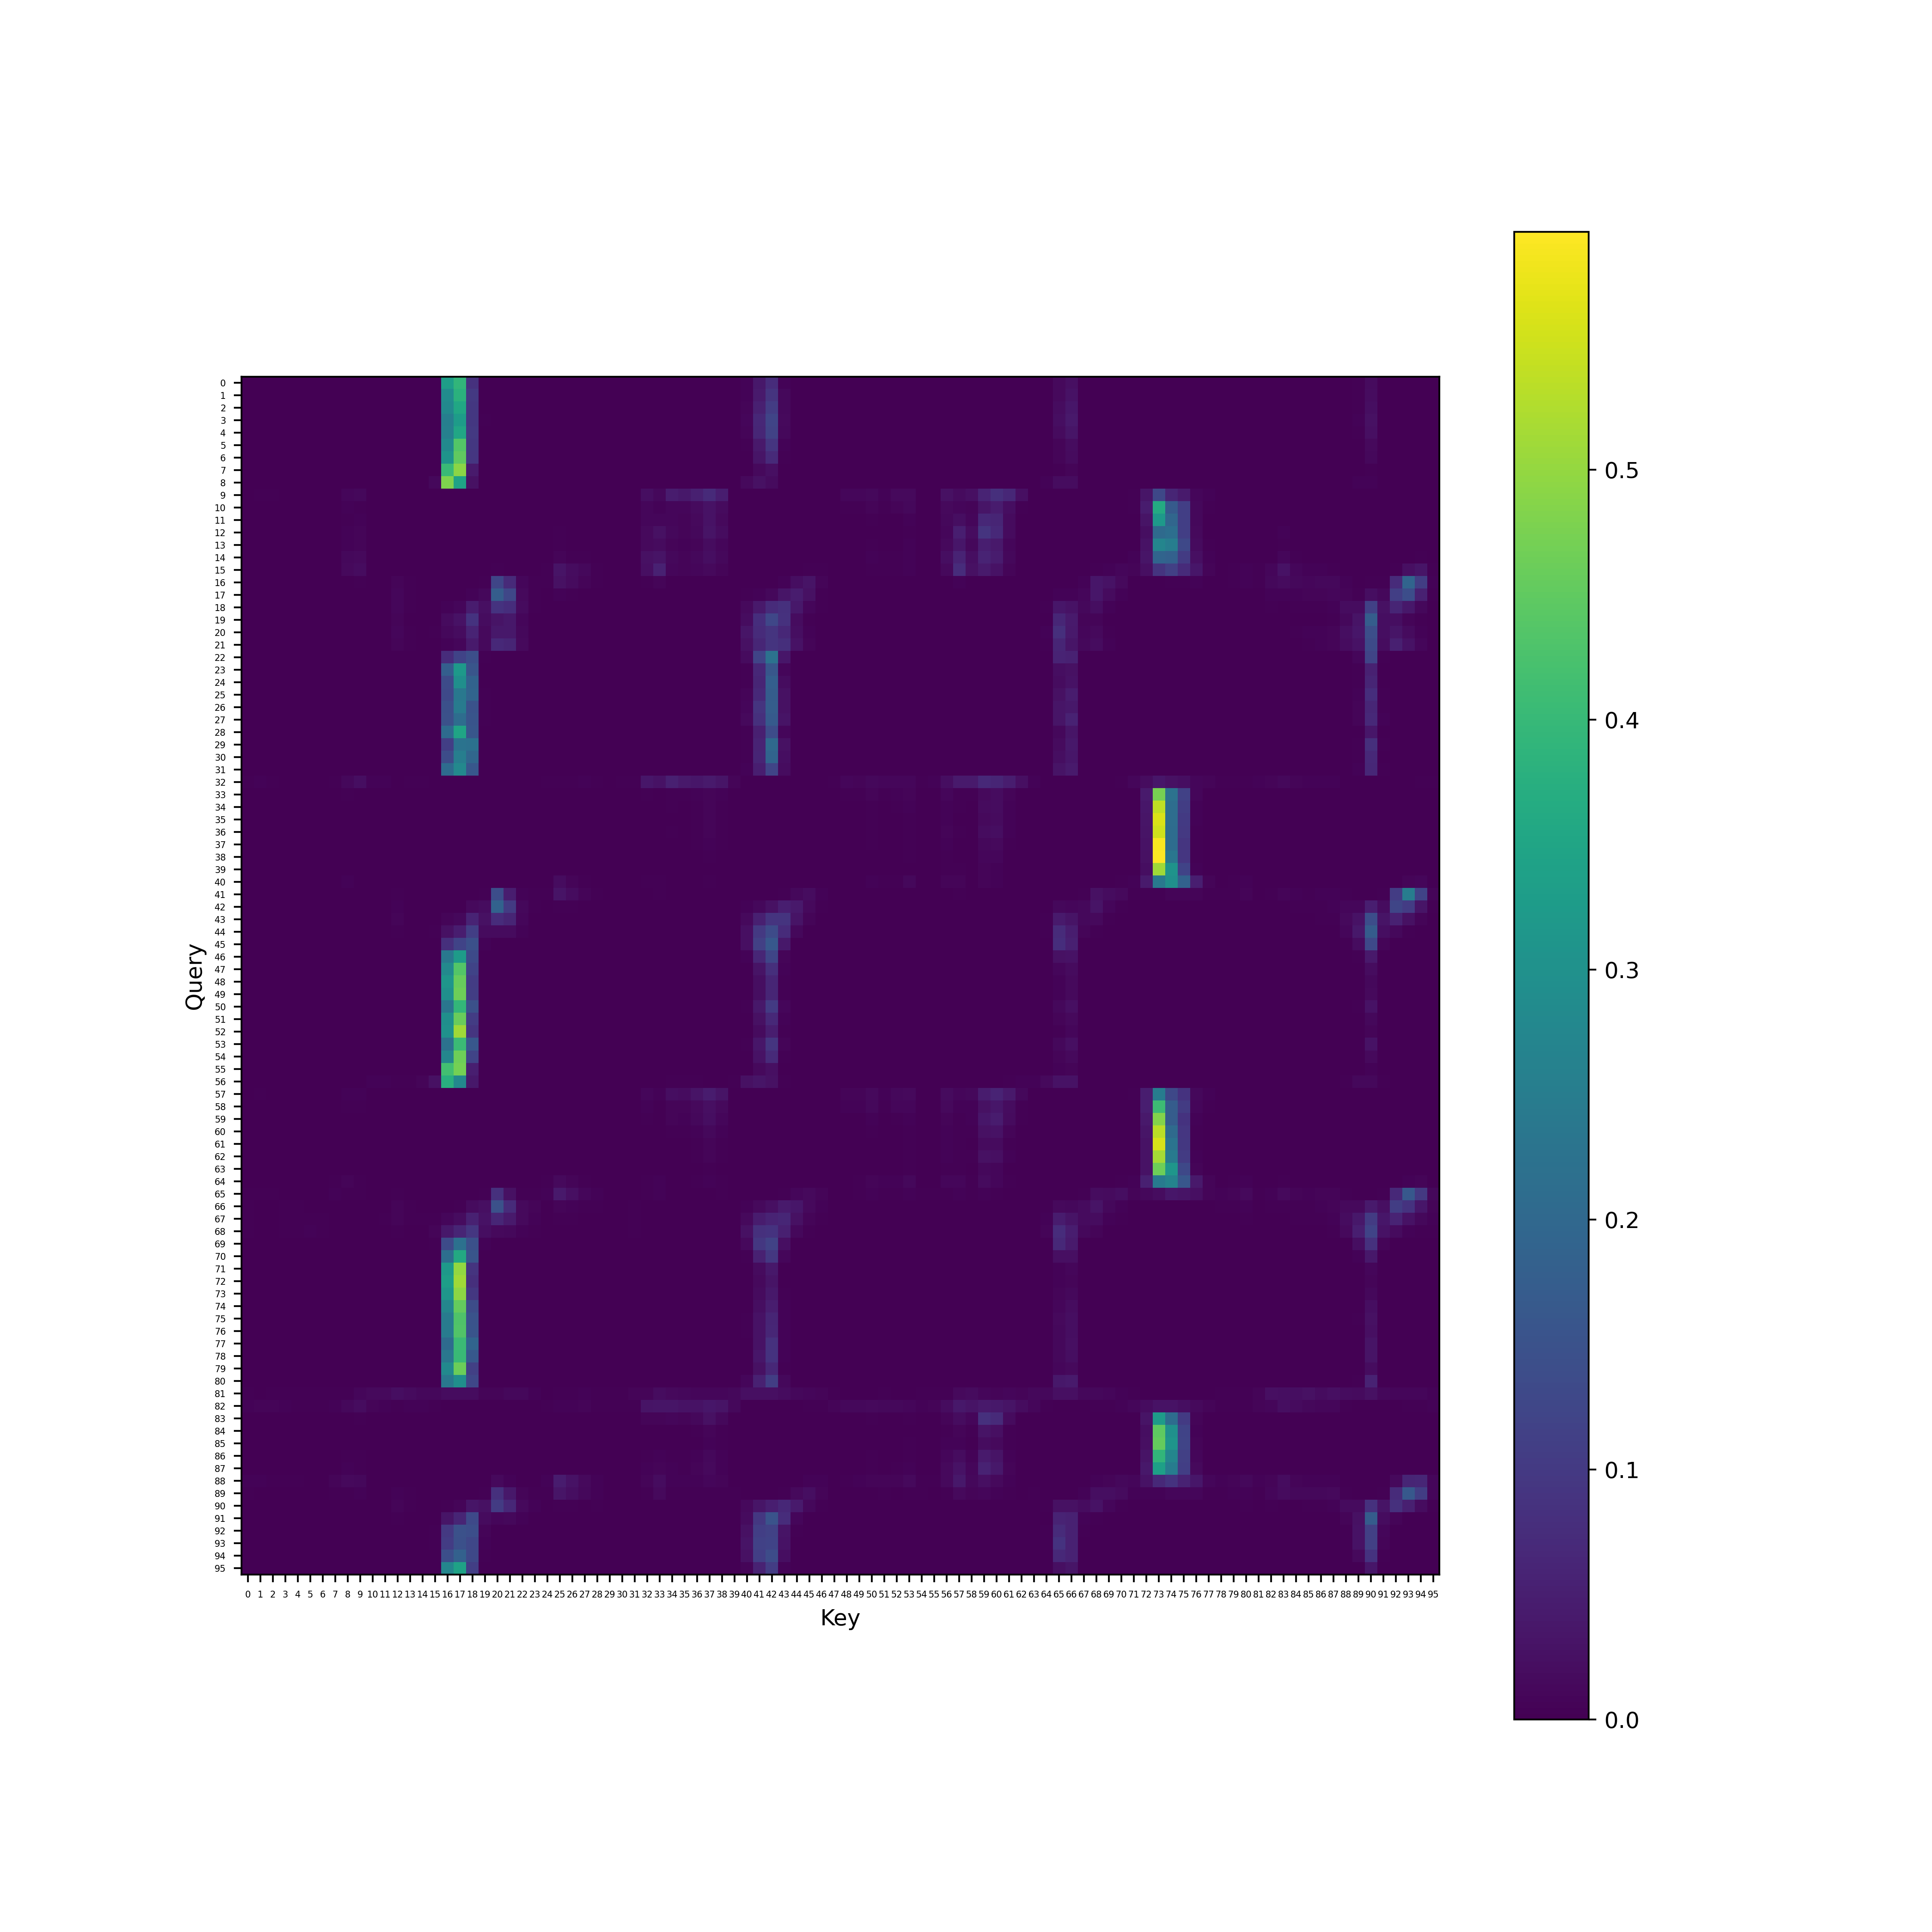
\includegraphics[width=0.48\columnwidth]{./assets/Transformer/0.png}}
        \subfigure[id = 20]{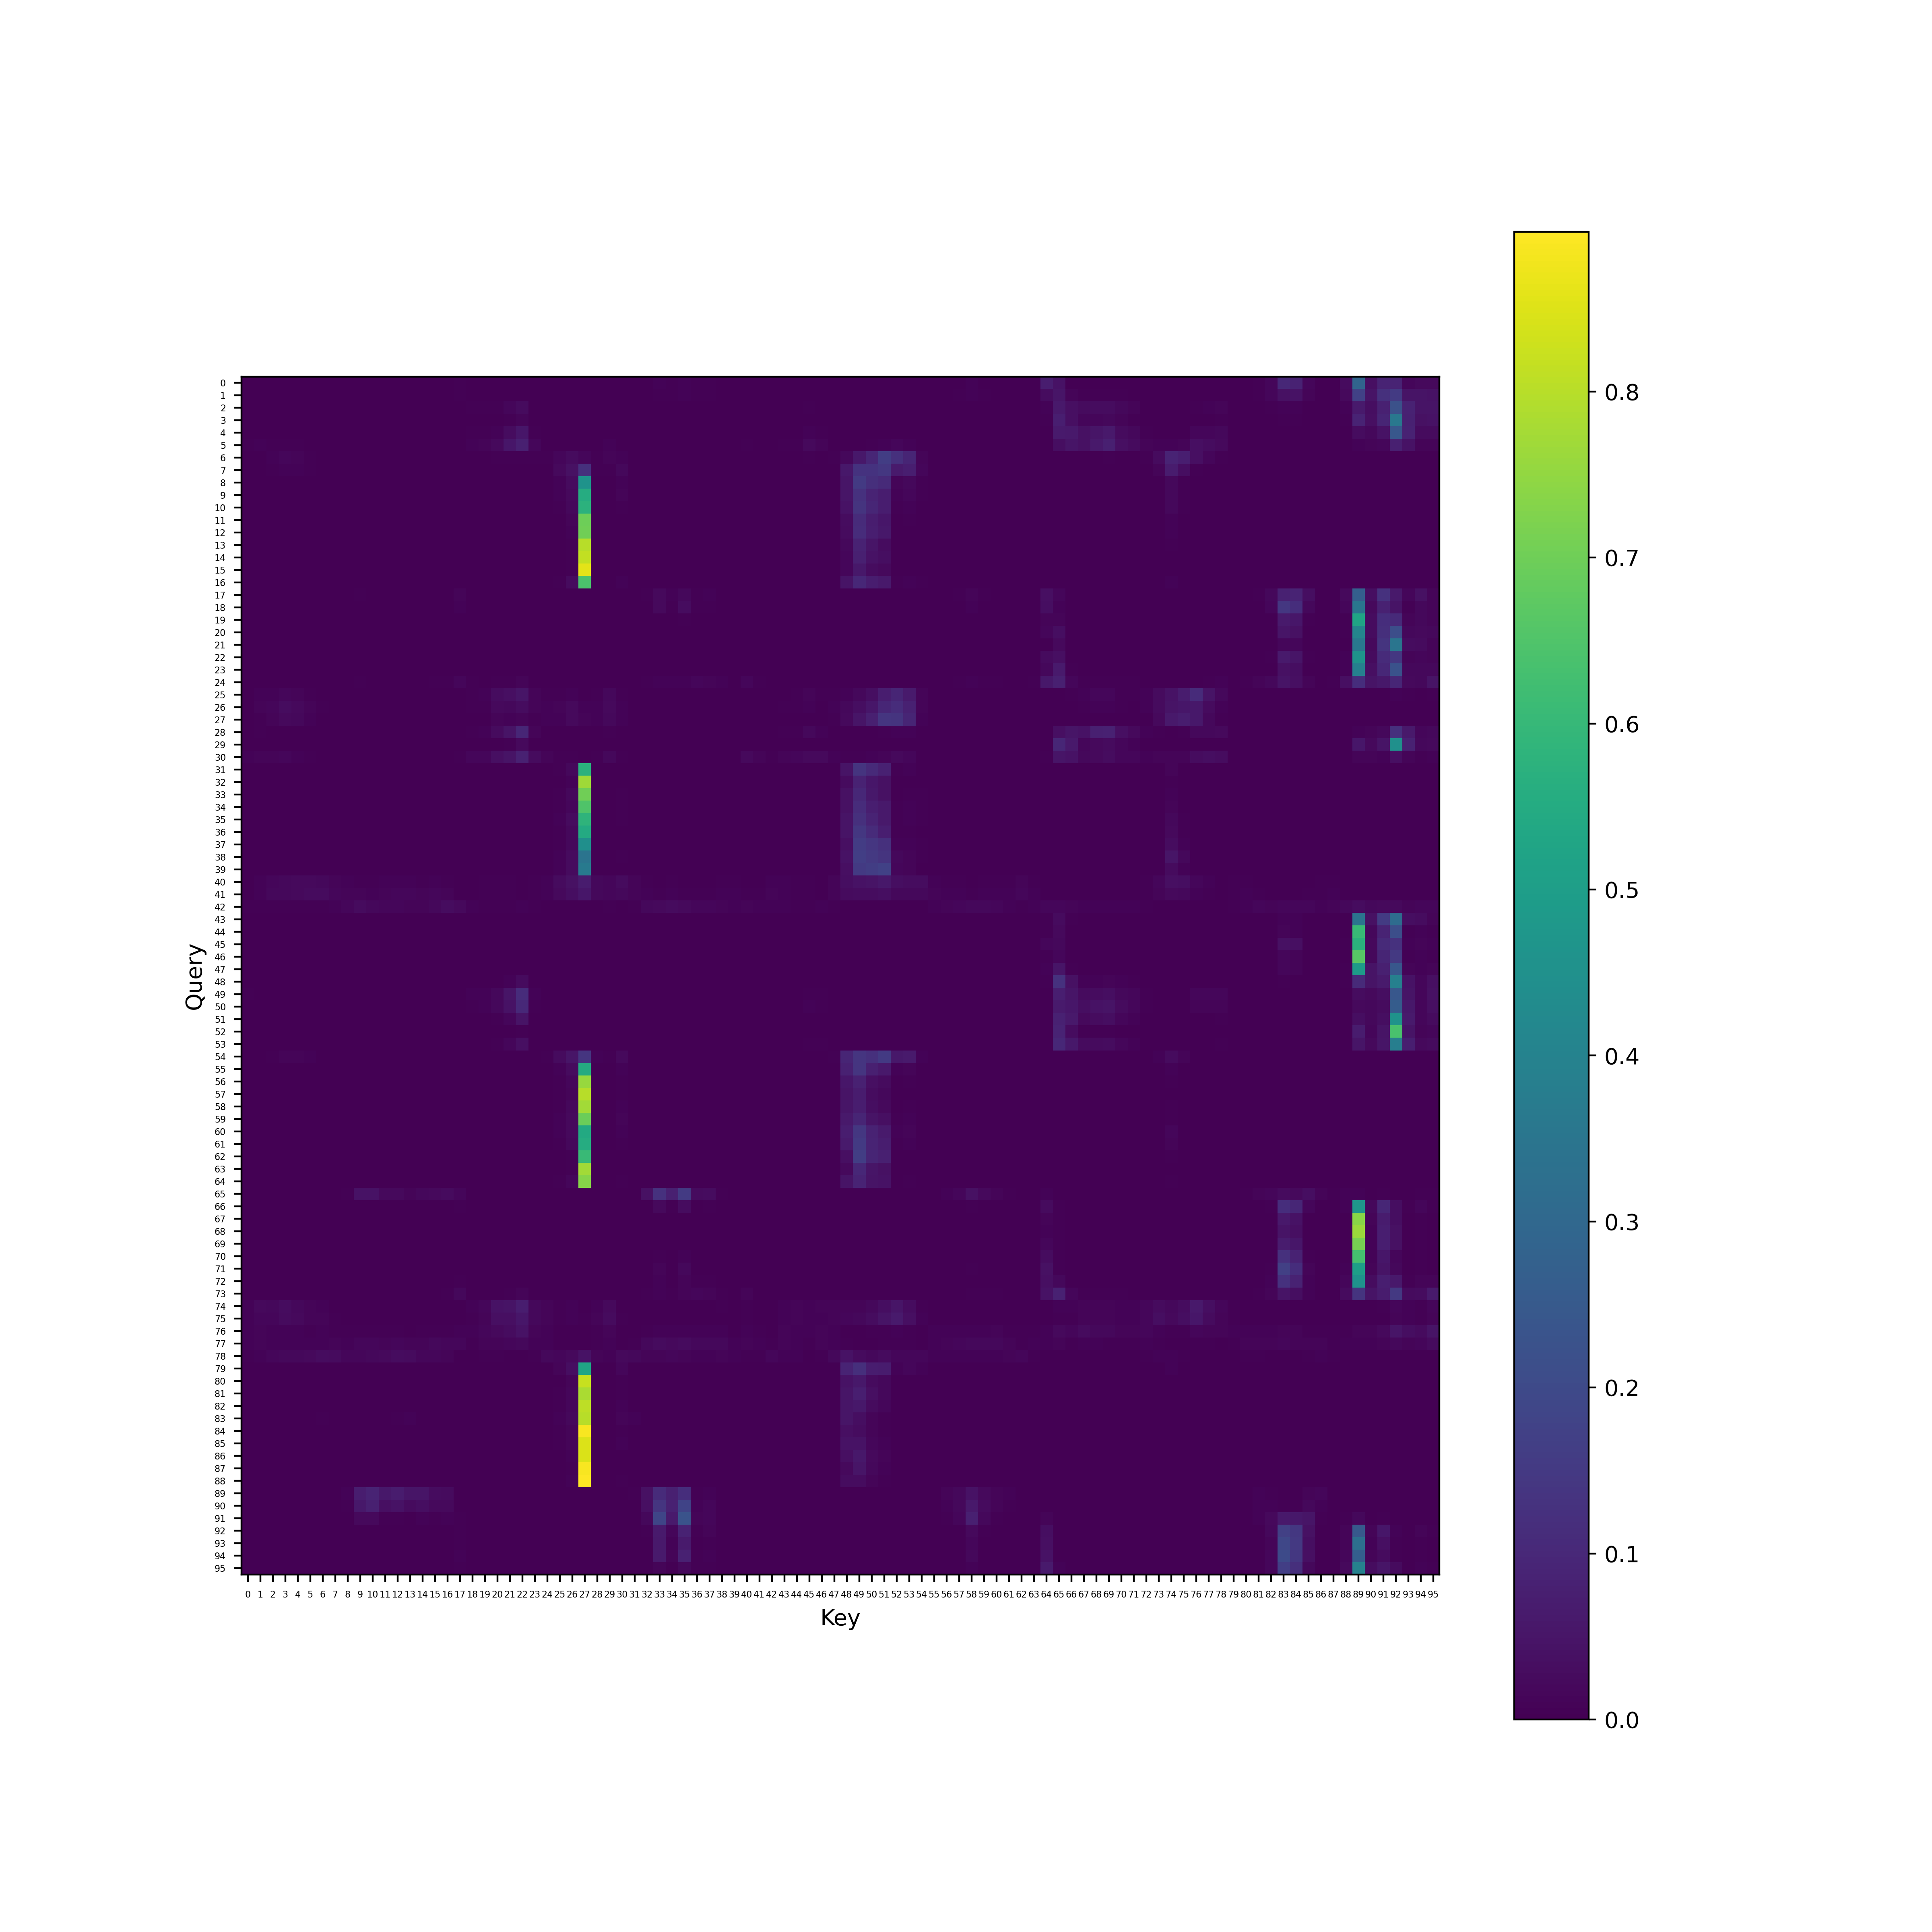
\includegraphics[width=0.48\columnwidth]{./assets/Transformer/20.png}}
        \subfigure[id = 40]{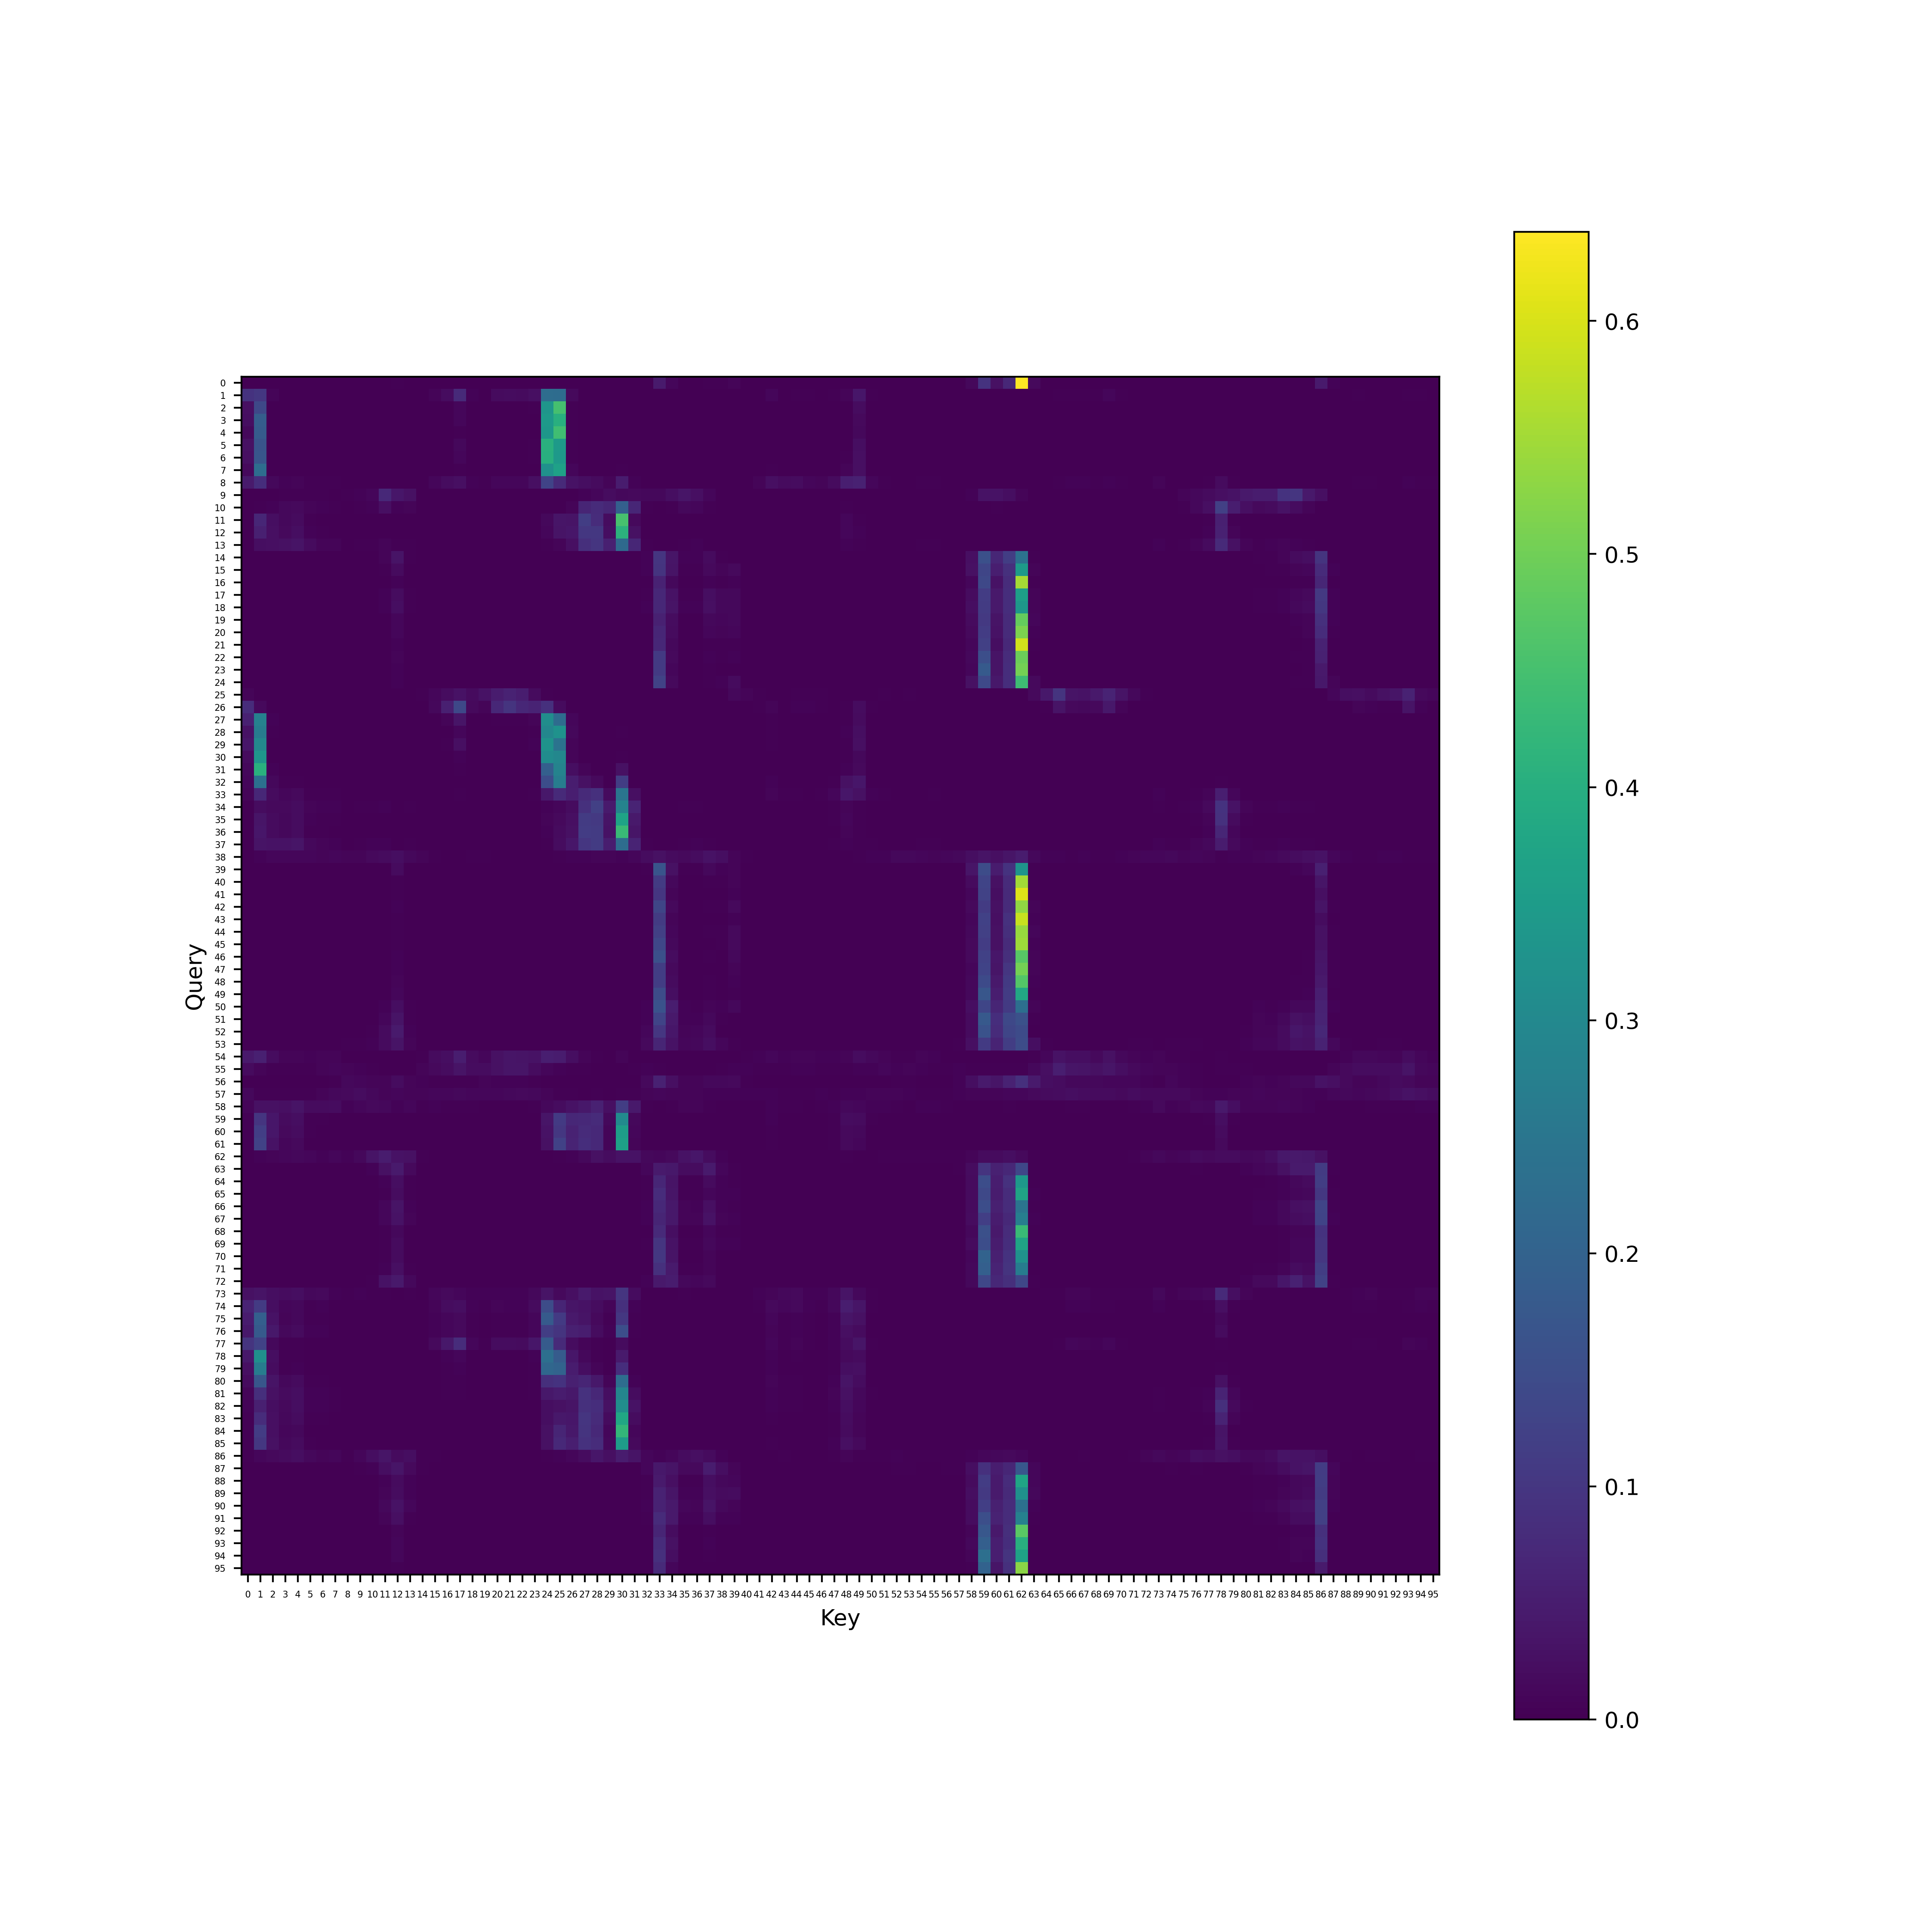
\includegraphics[width=0.48\columnwidth]{./assets/Transformer/40.png}}
        \subfigure[id = 60]{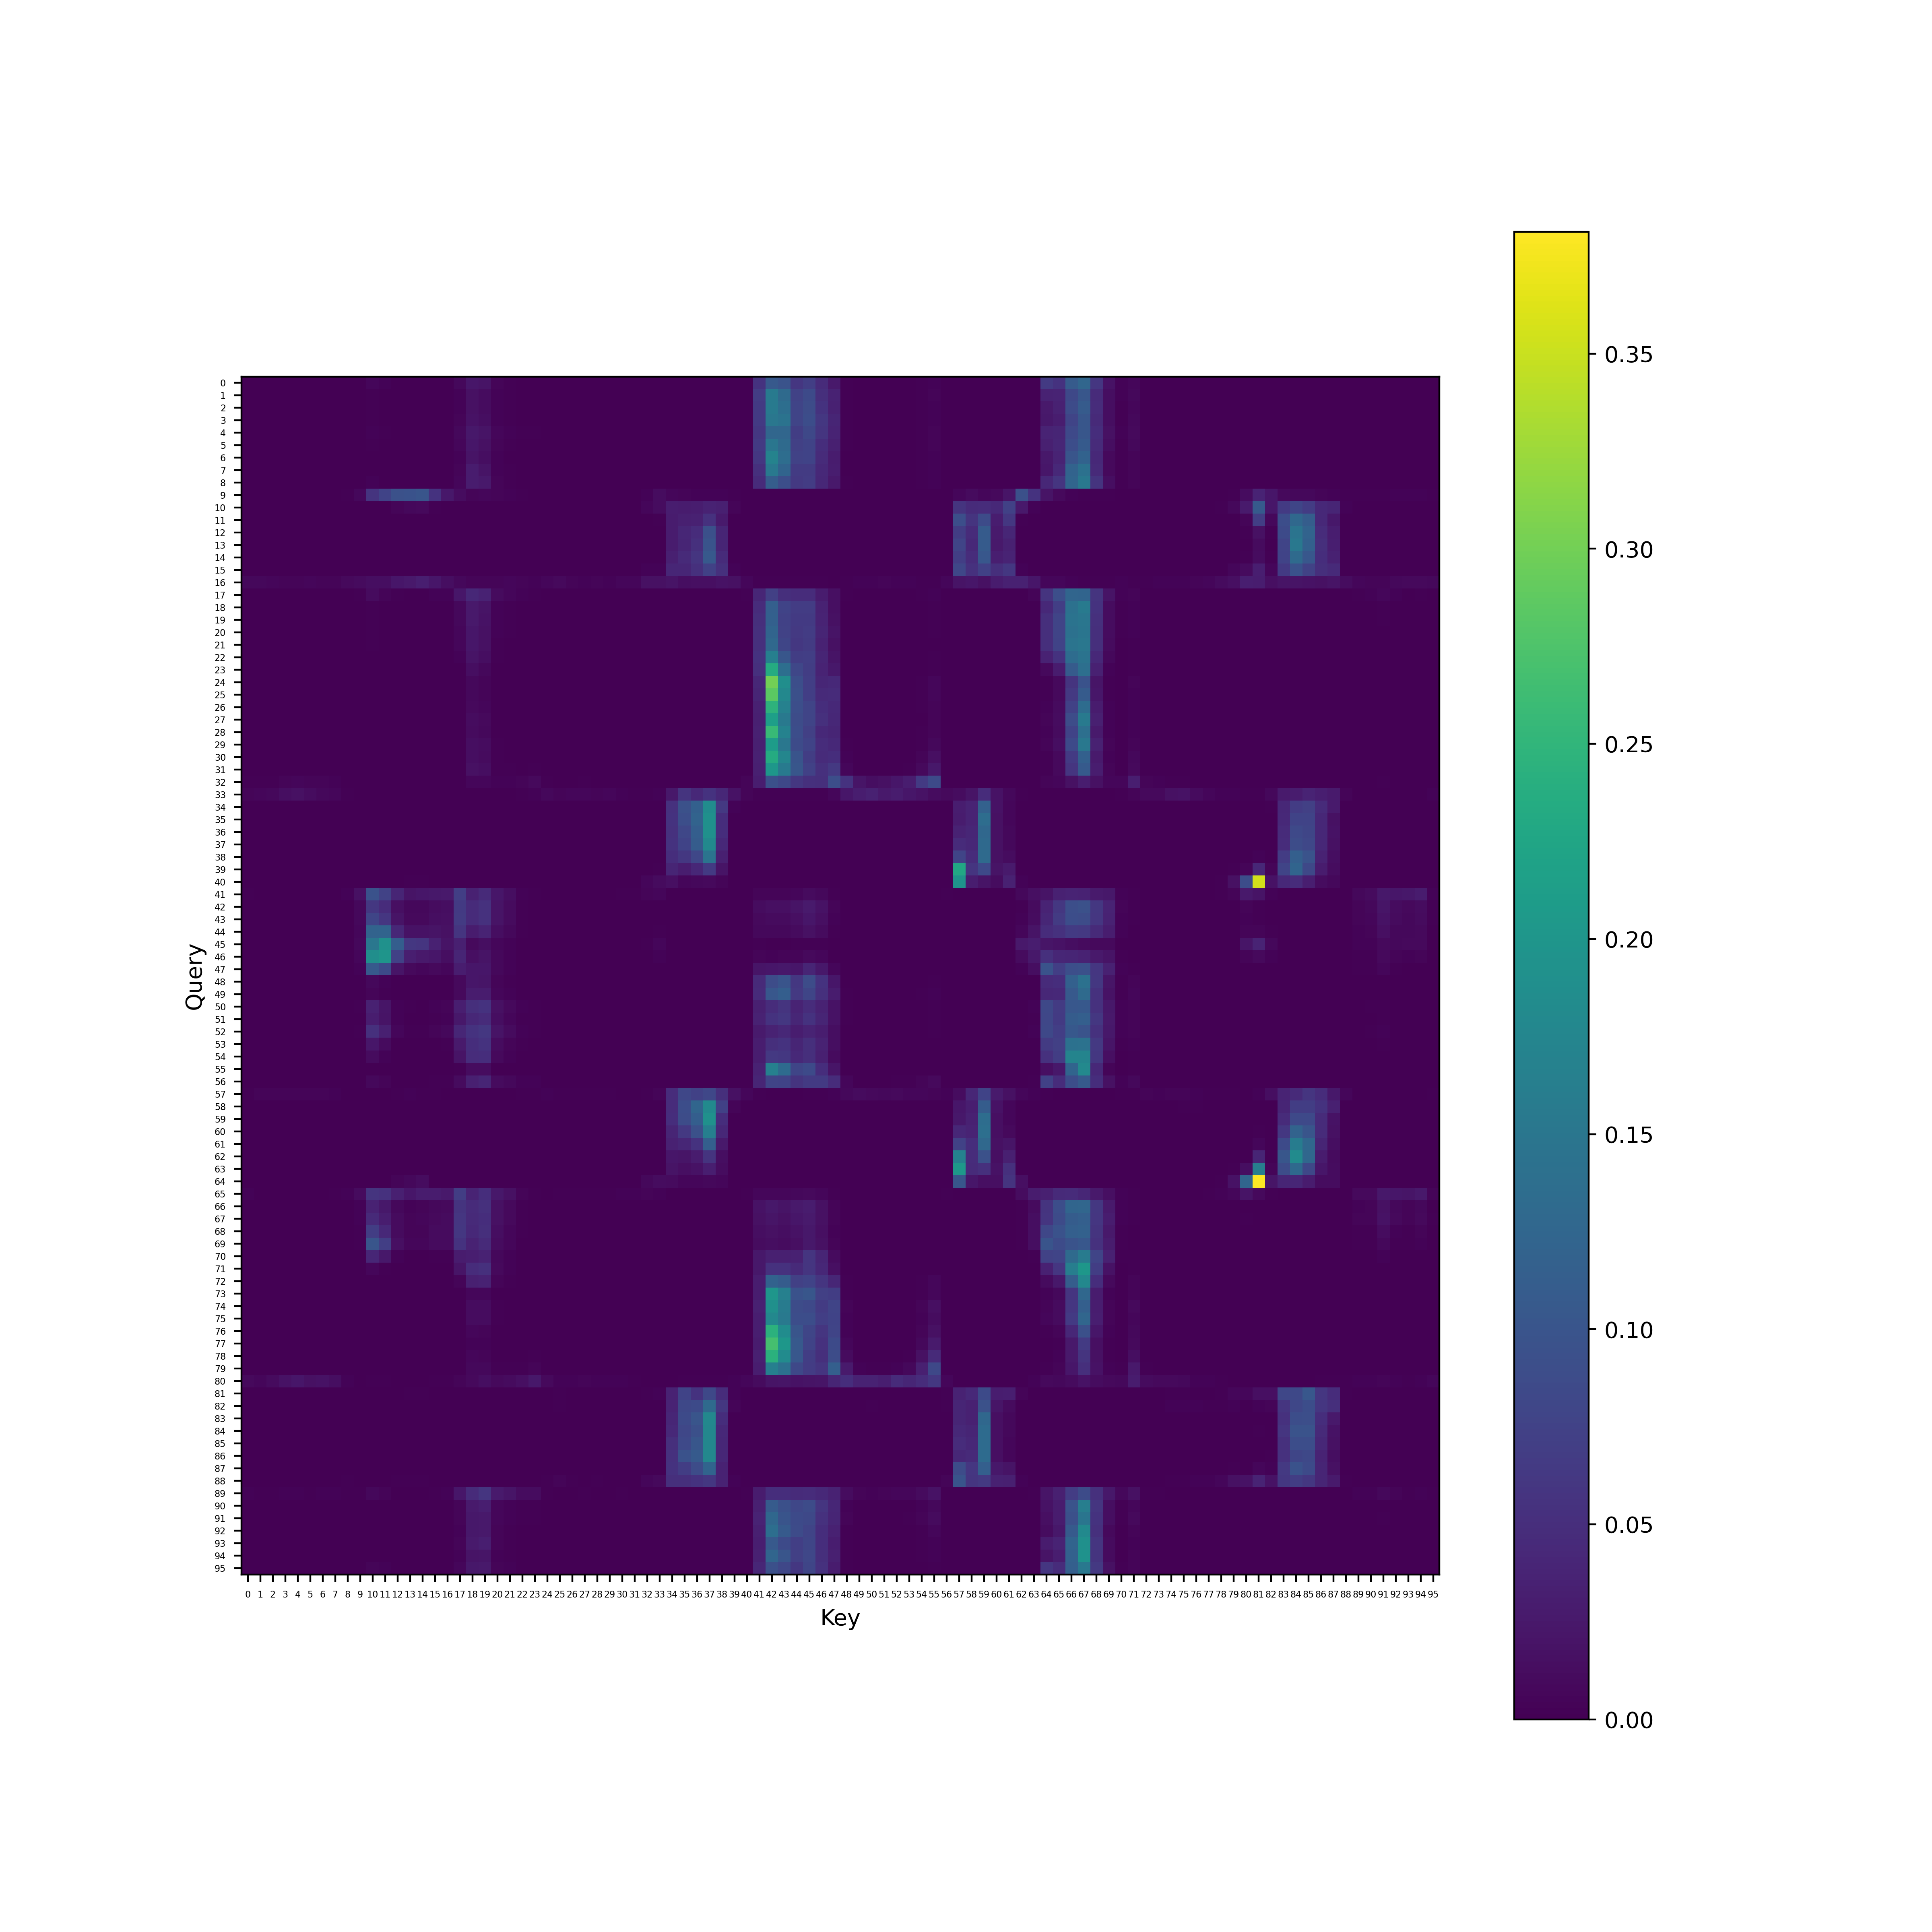
\includegraphics[width=0.48\columnwidth]{./assets/Transformer/60.png}}
        \caption{注意力的热力图可视化结果}
        \end{figure}

        图3的热力图和图2的预测结果是相对应的。我们发现，Transformer模型确实学习到了一些相关性特征。
        具体而言，在热力图中，每间隔一定距离，key和query就具有较大的attention值，说明它们具有较强的相关性。

        这意味着我们的预测对象——electricity，体现出了明显的周期性：每隔一定时长（约为24h）的历史数据对于当前值的影响较为显著，
        而其他时间的历史数据与当前值的相关性则相对较小。

    \subsection{Task4: Extra Techniques}

        在使用标准Transformer模型时，我们发现训练时间较长。
        这是因为标准Transformer模型的复杂度正比于与序列长度的平方，在输入序列的规模增大时，效率会迅速降低。

        参考相关论文，我采用了基于Local Attention的改进方式。 \endnote{Child, R., Gray, S., Radford, A., \& Sutskever, I. (2019). Generating long sequences with sparse transformers. arXiv preprint arXiv:1904.10509}
        Local Attention是Sparse Attention的一种实现，在训练和推理时只对临近的48个元素（即本例中最大序列长度的一半）计算attention，可以有效地提高Transformer模型的训练与推理效率。

        相关代码实现参见./Transformer/layers/attention.py的106-109行。

        训练过程中，模型在训练集、测试集和验证集上的loss变化曲线如图2所示。

        \begin{figure}[htbp]
        \centering
        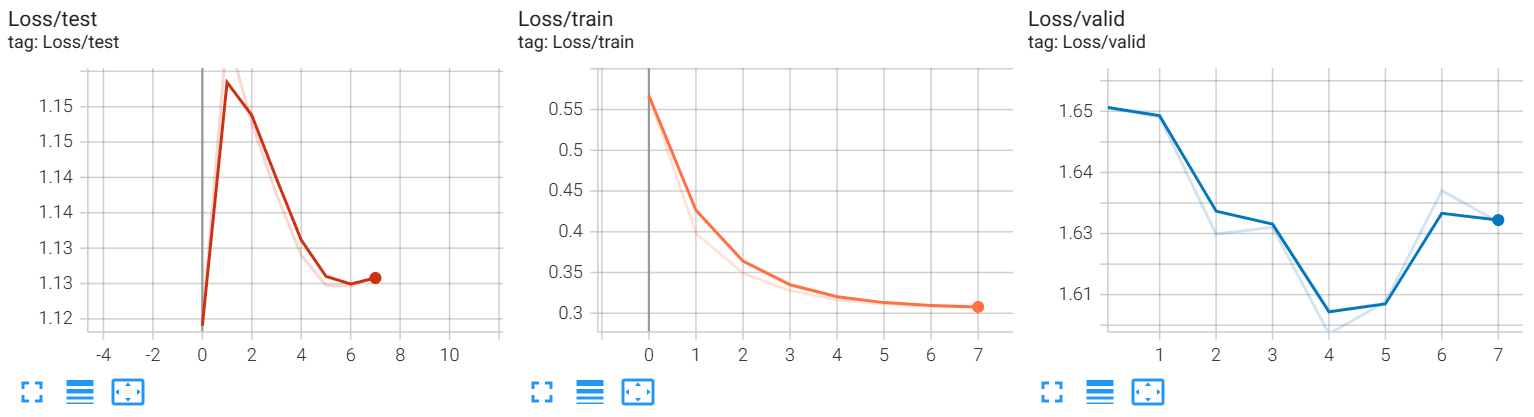
\includegraphics[width=1\textwidth]{./assets/Transformer/curve_st.png}
        \caption{改进模型在验证集、测试集和训练集上的loss变化曲线}
        \end{figure}

        如表1所示，我们尝试对比改进前后模型的训练用时和测试误差。

        \begin{table}[htbp]
        \caption{标准Transformer模型和改进Transformer模型的对比}
        \centering
        \begin{tabular}{cccc}
            \toprule
            model                & Time Cost &   MSE   &   MAE  \\
            \midrule
            Standard Transformer &   20 min  &  0.776  &  0.648 \\
            Sparse Transformer   &   12 min  &  0.928  &  0.713
        \end{tabular}
        \end{table}

        结果显示，在引入了Local Attention后，虽然模型的测试误差有微幅的提高，但训练的时间消耗显著降低，降低幅度将近一倍。
        综上，通过改进attention的计算方式，我们成功地提高了Transformer模型的效率，同时控制了精度损失在可接受的范围之内。

\section{Generative Adversarial Networks (GAN)}

\section{Diffusion Models}

    运行环境为：Ubuntu 22.04.3 LTS，Python 3.9.18，Tensorflow 2.15.0，PyTorch 2.1.2。

    \subsection{原理推导}

        \begin{enumerate}

        \item 证明：在$t \rightarrow \infty$时，$x_t$收敛至服从标准正态分布。

            我们引入服从正态分布的噪声参数$\epsilon \sim \NN(0, I)$，则前向扩散过程可以重参数为如下形式：
            \begin{align}
            x_t = \sqrt{1 - \beta_t} x_{t - 1} + \sqrt{\beta_t} \epsilon
            \end{align}

            记$\alpha_t = 1- \beta_t$，有：
            \begin{align*}
            x_t
            =& \sqrt{1 - \beta_t} x_{t - 1} + \beta_t \epsilon \\
            =& \sqrt{\alpha_t} x_{t - 1} + \sqrt{1 - \alpha_t} \epsilon \\
            =& \sqrt{\alpha_t} (\sqrt{\alpha_{t - 1}} x_{t - 2} + \sqrt{1 - \alpha_{t - 1}} \epsilon^\prime) + \sqrt{1 - \alpha_t} \epsilon \\
            =& \sqrt{\alpha_t \alpha_{t - 1}} x_{t - 2} + (\sqrt{\alpha_t - \alpha_t \alpha_{t - 1}} \epsilon^\prime + \sqrt{1 - \alpha_t} \epsilon)
            \end{align*}
            其中$\epsilon$和$\epsilon^\prime$是互相独立的标准正态分布随机变量，有：
            \begin{align*}
            (\sqrt{\alpha_t - \alpha_t \alpha_{t - 1}} \epsilon^\prime + \sqrt{1 - \alpha_t} \epsilon) \sim \NN(0, (1 - \alpha_t \alpha_{t - 1}) I)
            \end{align*}
            于是：
            \begin{align*}
            x_t
            =& \sqrt{\alpha_t \alpha_{t - 1}} x_{t - 2} + (\sqrt{\alpha_t - \alpha_t \alpha_{t - 1}} \epsilon^\prime + \sqrt{1 - \alpha_t} \epsilon) \\
            =& \sqrt{\alpha_t \alpha_{t - 1}} x_{t - 2} + \sqrt{1 - \alpha_t \alpha_{t - 1}} \epsilon \\
            =& ...... \\
            =& \sqrt{\prod \limits_{i=1}^{t} \alpha_i} \cdot x_0 + \sqrt{1 - \prod \limits_{i=1}^{t} \alpha_i} \cdot \epsilon
            \end{align*}

            在扩散模型中，我们选取了$\beta_t = c \in (0, 1]$，于是：$\alpha_t = 1 - \beta_t$的上界应严格小于$1$。
            因此，在$t \rightarrow \infty$时，$\prod \limits_{i=1}^{t} \alpha_i \rightarrow 0$，即有：
            \begin{align}
            x_t \rightarrow \epsilon \sim \NN(0, I)
            \end{align}

        \item 证明：后验分布$q(x_{t - 1} \vert x_t, x_0)$服从正态分布。

            使用Bayes公式：
            \begin{align*}
            q(x_{t - 1} \vert x_t, x_0)
            =& \frac{q(x_{t - 1}, x_t \vert x_0)}{q(x_t \vert x_0)} \\
            =& \frac{q(x_t \vert x_{t - 1}, x_0) q(x_{t - 1} \vert x_0)}{q(x_t \vert x_0)} \\
            =& \frac{q(x_t \vert x_{t - 1}) q(x_{t - 1} \vert x_0)}{q(x_t \vert x_0)}
            \end{align*}

            记$\al_t = \prod \limits_{i=1}^{t} \alpha_i$，
            我们已经证明：$q(x_t \vert x_0) = \NN (x_t; \sqrt{\al_t}, \sqrt{1 - \al_t} I)$，故：
            \begin{align*}
            &q(x_{t - 1} \vert x_t, x_0) \\
            =& \frac{q(x_t \vert x_{t - 1}) q(x_{t - 1} \vert x_0)}{q(x_t \vert x_0)} \\
            \varpropto& \exp\{\frac{(x_t - \sqrt{\alpha_t} x_{t - 1})^2}{2 (1 - \alpha_t)} + \frac{(x_{t - 1} + \sqrt{\al_{t - 1}})^2}{2 (1 - \al_{t - 1})} - \frac{(x_t - \sqrt{\al_t})^2}{2 (1 - \al_t)}\} \\
            =& \exp\{-\frac{1}{2} [\frac{1 - \al_t}{(1 - \alpha_t)(1 - \al_{t - 1})} x_{t - 1}^2 - 2(\frac{\sqrt{\alpha_t} x_t}{1 - \alpha_t} + \frac{\sqrt{\al_{t - 1}} x_0}{1 - \al_{t - 1}}) x_{t - 1} + C]\}
            \end{align*}
            其中$C = C(x_t, x_0)$，是与$x_{t - 1}$无关的常量。于是：
            \begin{align*}
            &q(x_{t - 1} \vert x_t, x_0) \\
            \sim& \exp\{-\frac{1}{2} [\frac{(x_{t - 1} - \frac{\sqrt{\alpha_t} (1 - \al_{t - 1}) x_t + \sqrt{\al_{t - 1}} (1 - \alpha_t) x_0}{1 - \al_t})^2}{(\sqrt{\frac{(1 - \alpha_t) (1 - \al_{t - 1})}{1 - \al_t}})^2}]\} \\
            \sim& \NN(x_{t - 1}; \frac{\sqrt{\alpha_t} (1 - \al_{t - 1}) x_t + \sqrt{\al_{t - 1}} (1 - \alpha_t) x_0}{1 - \al_t}, \frac{(1 - \alpha_t) (1 - \al_{t - 1})}{1 - \al_t} I)
            \end{align*}
            对$q(x_{t - 1} \vert x_t, x_0)$归一化，：
            \begin{align*}
            &q(x_{t - 1} \vert x_t, x_0) \\
            =& \NN(x_{t - 1}; \frac{\sqrt{\alpha_t} (1 - \al_{t - 1}) x_t + \sqrt{\al_{t - 1}} (1 - \alpha_t) x_0}{1 - \al_t}, \frac{(1 - \alpha_t) (1 - \al_{t - 1})}{1 - \al_t} I)
            \end{align*}

            综上，$q(x_{t - 1} \vert x_t, x_0)$服从正态分布$\NN(\tilde{u}_t, \tilde{\beta}_t I)$，其中均值$\tilde{u}_t$、方差$\tilde{\beta}_t$为：
            \begin{align}
            \tilde{u}_t =& \frac{\sqrt{\alpha_t} (1 - \al_{t - 1}) x_t + \sqrt{\al_{t - 1}} (1 - \alpha_t) x_0}{1 - \al_t} \\
            \tilde{\beta}_t =& \frac{(1 - \alpha_t) (1 - \al_{t - 1})}{1 - \al_t}
            \end{align}

        \end{enumerate}

    \subsection{DDPM}

        调整classifier\_sample.sh中的diffusion\_steps参数，基于DDPM生成的图像如图5所示。
        同时，我们还记录了生成图片在ImageNet中的类别名称，以供参考。

        \begin{figure}[htbp]
        \centering
        \subfigure[steps=2, Persian Cat]{\includegraphics[width=0.32\columnwidth]{./assets/DDPM/image\_sample\_2\_283.png}}
        \subfigure[steps=4, Nile Crocodile]{\includegraphics[width=0.32\columnwidth]{./assets/DDPM/image\_sample\_4\_49.png}}
        \subfigure[steps=8, Backpack]{\includegraphics[width=0.32\columnwidth]{./assets/DDPM/image\_sample\_8\_414.png}}
        \subfigure[steps=16, Fox Terrier]{\includegraphics[width=0.32\columnwidth]{./assets/DDPM/image\_sample\_16\_188.png}}
        \subfigure[steps=32, Goldfinch]{\includegraphics[width=0.32\columnwidth]{./assets/DDPM/image\_sample\_32\_11.png}}
        \subfigure[steps=64, Dome]{\includegraphics[width=0.32\columnwidth]{./assets/DDPM/image\_sample\_64\_538.png}}
        \subfigure[steps=128, Helmet]{\includegraphics[width=0.32\columnwidth]{./assets/DDPM/image\_sample\_128\_560.png}}
        \subfigure[steps=256, Lemon]{\includegraphics[width=0.32\columnwidth]{./assets/DDPM/image\_sample\_256\_951.png}}
        \subfigure[steps=512, Tow Truck]{\includegraphics[width=0.32\columnwidth]{./assets/DDPM/image\_sample\_512\_864.png}}
        \subfigure[steps=1000, Tank]{\includegraphics[width=0.32\columnwidth]{./assets/DDPM/image\_sample\_1000\_847.png}}
        \subfigure[steps=1024, Hen]{\includegraphics[width=0.32\columnwidth]{./assets/DDPM/image\_sample\_1024\_8.png}}
        \subfigure[steps=2048, Yawl]{\includegraphics[width=0.32\columnwidth]{./assets/DDPM/image\_sample\_2048\_914.png}}
        \caption{DDPM在不同diffusion\_steps参数下生成的图片示例}
        \end{figure}

        可以看出，DDPM能够成功生成符合一般认知逻辑的图片，其内容也与ImageNet中的类别名称相符合。

        通过调整diffusion\_steps参数，我们发现：
        在采样步数小于64步时，DDPM生成的图片开始变得模糊；在采样步数小于8步时，DDPM生成的图片已无法辨识。
        而当采样步数过大时（大于256步），图片的清晰度并没有较为明显的提升。因此，考虑到生成效率的问题，
        我们认为取diffusion\_steps为256-512较为合适。

    \subsection{DDIM}

        仿造GaussianDiffusion类中p\_sample方法和p\_mean\_variance方法，并参考课件86页给出的公式，我们补全了DDIM的sampler。 \endnote{Song, J., Meng, C., \& Ermon, S. (2021). Denoising diffusion implicit models. In Proceedings of the 9th International Conference on Learning Representations (pp. 1-18)}
        源代码参见./Diffusion/guided\_diffusion/gaussian\_diffusion.py中的ddim\_sample方法和p\_mean\_variance\_ddim方法。
        另外，注意到在实际调用模型时，p\_mean\_variance\_ddim方法还需要在子类SpacedDiffusion重写，
        此部分参见./Diffusion/guided\_diffusion/respace.py中SpacedDiffusion类的实现。

        调整diffusion\_steps参数，基于DDIM生成的图像及其类别名称如图6所示。

        \begin{figure}[htbp]
        \centering
        \subfigure[steps=2, Butcher Shop]{\includegraphics[width=0.32\columnwidth]{./assets/DDIM/image\_sample\_2\_467.png}}
        \subfigure[steps=4, Welsh Spaniel]{\includegraphics[width=0.32\columnwidth]{./assets/DDIM/image\_sample\_4\_218.png}}
        \subfigure[steps=8, Heron]{\includegraphics[width=0.32\columnwidth]{./assets/DDIM/image\_sample\_8\_131.png}}
        \subfigure[steps=16, Oil Filter]{\includegraphics[width=0.32\columnwidth]{./assets/DDIM/image\_sample\_16\_686.png}}
        \subfigure[steps=32, Weimaraner]{\includegraphics[width=0.32\columnwidth]{./assets/DDIM/image\_sample\_32\_178.png}}
        \subfigure[steps=64, Frypan]{\includegraphics[width=0.32\columnwidth]{./assets/DDIM/image\_sample\_64\_567.png}}
        \subfigure[steps=128, Peacock]{\includegraphics[width=0.32\columnwidth]{./assets/DDIM/image\_sample\_128\_84.png}}
        \subfigure[steps=256, Maillot]{\includegraphics[width=0.32\columnwidth]{./assets/DDIM/image\_sample\_256\_638.png}}
        \subfigure[steps=512, Merganser]{\includegraphics[width=0.32\columnwidth]{./assets/DDIM/image\_sample\_512\_98.png}}
        \subfigure[steps=1000, Tank]{\includegraphics[width=0.32\columnwidth]{./assets/DDIM/image\_sample\_1000\_847.png}}
        \subfigure[steps=1024, Convertible]{\includegraphics[width=0.32\columnwidth]{./assets/DDIM/image\_sample\_1024\_511.png}}
        \subfigure[steps=2048, Kimono]{\includegraphics[width=0.32\columnwidth]{./assets/DDIM/image\_sample\_2048\_614.png}}
        \caption{DDIM在不同diffusion\_steps参数下生成的图片示例}
        \end{figure}

        可以看出，DDIM的生成效果同样较好。
        在采样步数大于128步时，DDIM和DDPM的生成效果几乎没有区别，都可以生成与类别名称相符合的低噪图像。

        注意到，在采样步数小于128步时（16步、32步和64步），在DDIM的生成图像中开始出现明显的噪点。
        对比而言，在同样的采样步数下，DDPM的生成图像的质量同样有所下降。
        二者在直观表现上存在一定的区别。
        DDIM的生成图像整体上仍然较为清晰，但噪点更多、更密集；
        而在DDPM的生成图像中并没有观察到明显的噪点，但整体的清晰度更低。

        进一步降低采样步数，在采样步数小于16时，DDPM的生成图像已经几乎无法辨识。
        而在DDIM的生成图像中，虽然存在大量噪点，但仍然能够大致辨认出图像的类别。

    \subsection{CGDM}

        设置class\_index=847，我们希望模型生成类别为“坦克”的图片。

        固定diffusion\_steps=512，使用DDPM，
        我们调整classifier\_scale参数的值，观察模型生成图片的效果，结果如图7-图11所示。

        \begin{figure}[htbp]
        \centering
        \subfigure{\includegraphics[width=0.19\columnwidth]{./assets/CGDM/scale=1e+2/image\_sample0\_1.png}}
        \subfigure{\includegraphics[width=0.19\columnwidth]{./assets/CGDM/scale=1e+2/image\_sample0\_2.png}}
        \subfigure{\includegraphics[width=0.19\columnwidth]{./assets/CGDM/scale=1e+2/image\_sample0\_3.png}}
        \subfigure{\includegraphics[width=0.19\columnwidth]{./assets/CGDM/scale=1e+2/image\_sample0\_4.png}}
        \subfigure{\includegraphics[width=0.19\columnwidth]{./assets/CGDM/scale=1e+2/image\_sample0\_5.png}}
        \subfigure{\includegraphics[width=0.19\columnwidth]{./assets/CGDM/scale=1e+2/image\_sample0\_6.png}}
        \subfigure{\includegraphics[width=0.19\columnwidth]{./assets/CGDM/scale=1e+2/image\_sample0\_7.png}}
        \subfigure{\includegraphics[width=0.19\columnwidth]{./assets/CGDM/scale=1e+2/image\_sample0\_8.png}}
        \subfigure{\includegraphics[width=0.19\columnwidth]{./assets/CGDM/scale=1e+2/image\_sample0\_9.png}}
        \subfigure{\includegraphics[width=0.19\columnwidth]{./assets/CGDM/scale=1e+2/image\_sample0\_10.png}}
        \subfigure{\includegraphics[width=0.19\columnwidth]{./assets/CGDM/scale=1e+2/image\_sample0\_11.png}}
        \subfigure{\includegraphics[width=0.19\columnwidth]{./assets/CGDM/scale=1e+2/image\_sample0\_12.png}}
        \subfigure{\includegraphics[width=0.19\columnwidth]{./assets/CGDM/scale=1e+2/image\_sample0\_13.png}}
        \subfigure{\includegraphics[width=0.19\columnwidth]{./assets/CGDM/scale=1e+2/image\_sample0\_14.png}}
        \subfigure{\includegraphics[width=0.19\columnwidth]{./assets/CGDM/scale=1e+2/image\_sample0\_15.png}}
        \caption{CGDM的生成图像, 指定生成类别为847(Tank), classifier\_scale=100}
        \end{figure}

        \begin{figure}[htbp]
        \centering
        \subfigure{\includegraphics[width=0.19\columnwidth]{./assets/CGDM/scale=1e+1/image\_sample0\_1.png}}
        \subfigure{\includegraphics[width=0.19\columnwidth]{./assets/CGDM/scale=1e+1/image\_sample0\_2.png}}
        \subfigure{\includegraphics[width=0.19\columnwidth]{./assets/CGDM/scale=1e+1/image\_sample0\_3.png}}
        \subfigure{\includegraphics[width=0.19\columnwidth]{./assets/CGDM/scale=1e+1/image\_sample0\_4.png}}
        \subfigure{\includegraphics[width=0.19\columnwidth]{./assets/CGDM/scale=1e+1/image\_sample0\_5.png}}
        \subfigure{\includegraphics[width=0.19\columnwidth]{./assets/CGDM/scale=1e+1/image\_sample0\_6.png}}
        \subfigure{\includegraphics[width=0.19\columnwidth]{./assets/CGDM/scale=1e+1/image\_sample0\_7.png}}
        \subfigure{\includegraphics[width=0.19\columnwidth]{./assets/CGDM/scale=1e+1/image\_sample0\_8.png}}
        \subfigure{\includegraphics[width=0.19\columnwidth]{./assets/CGDM/scale=1e+1/image\_sample0\_9.png}}
        \subfigure{\includegraphics[width=0.19\columnwidth]{./assets/CGDM/scale=1e+1/image\_sample0\_10.png}}
        \subfigure{\includegraphics[width=0.19\columnwidth]{./assets/CGDM/scale=1e+1/image\_sample0\_11.png}}
        \subfigure{\includegraphics[width=0.19\columnwidth]{./assets/CGDM/scale=1e+1/image\_sample0\_12.png}}
        \subfigure{\includegraphics[width=0.19\columnwidth]{./assets/CGDM/scale=1e+1/image\_sample0\_13.png}}
        \subfigure{\includegraphics[width=0.19\columnwidth]{./assets/CGDM/scale=1e+1/image\_sample0\_14.png}}
        \subfigure{\includegraphics[width=0.19\columnwidth]{./assets/CGDM/scale=1e+1/image\_sample0\_15.png}}
        \caption{CGDM的生成图像：指定生成类别为847(Tank), classifier\_scale=10}
        \end{figure}

        \begin{figure}[htbp]
        \centering
        \subfigure{\includegraphics[width=0.19\columnwidth]{./assets/CGDM/scale=1/image\_sample0\_1.png}}
        \subfigure{\includegraphics[width=0.19\columnwidth]{./assets/CGDM/scale=1/image\_sample0\_2.png}}
        \subfigure{\includegraphics[width=0.19\columnwidth]{./assets/CGDM/scale=1/image\_sample0\_3.png}}
        \subfigure{\includegraphics[width=0.19\columnwidth]{./assets/CGDM/scale=1/image\_sample0\_4.png}}
        \subfigure{\includegraphics[width=0.19\columnwidth]{./assets/CGDM/scale=1/image\_sample0\_5.png}}
        \subfigure{\includegraphics[width=0.19\columnwidth]{./assets/CGDM/scale=1/image\_sample0\_6.png}}
        \subfigure{\includegraphics[width=0.19\columnwidth]{./assets/CGDM/scale=1/image\_sample0\_7.png}}
        \subfigure{\includegraphics[width=0.19\columnwidth]{./assets/CGDM/scale=1/image\_sample0\_8.png}}
        \subfigure{\includegraphics[width=0.19\columnwidth]{./assets/CGDM/scale=1/image\_sample0\_9.png}}
        \subfigure{\includegraphics[width=0.19\columnwidth]{./assets/CGDM/scale=1/image\_sample0\_10.png}}
        \subfigure{\includegraphics[width=0.19\columnwidth]{./assets/CGDM/scale=1/image\_sample0\_11.png}}
        \subfigure{\includegraphics[width=0.19\columnwidth]{./assets/CGDM/scale=1/image\_sample0\_12.png}}
        \subfigure{\includegraphics[width=0.19\columnwidth]{./assets/CGDM/scale=1/image\_sample0\_13.png}}
        \subfigure{\includegraphics[width=0.19\columnwidth]{./assets/CGDM/scale=1/image\_sample0\_14.png}}
        \subfigure{\includegraphics[width=0.19\columnwidth]{./assets/CGDM/scale=1/image\_sample0\_15.png}}
        \caption{CGDM的生成图像：指定生成类别为847(Tank), classifier\_scale=1}
        \end{figure}

        \begin{figure}[htbp]
        \centering
        \subfigure{\includegraphics[width=0.19\columnwidth]{./assets/CGDM/scale=1e-2/image\_sample0\_1.png}}
        \subfigure{\includegraphics[width=0.19\columnwidth]{./assets/CGDM/scale=1e-2/image\_sample0\_2.png}}
        \subfigure{\includegraphics[width=0.19\columnwidth]{./assets/CGDM/scale=1e-2/image\_sample0\_3.png}}
        \subfigure{\includegraphics[width=0.19\columnwidth]{./assets/CGDM/scale=1e-2/image\_sample0\_4.png}}
        \subfigure{\includegraphics[width=0.19\columnwidth]{./assets/CGDM/scale=1e-2/image\_sample0\_5.png}}
        \subfigure{\includegraphics[width=0.19\columnwidth]{./assets/CGDM/scale=1e-2/image\_sample0\_6.png}}
        \subfigure{\includegraphics[width=0.19\columnwidth]{./assets/CGDM/scale=1e-2/image\_sample0\_7.png}}
        \subfigure{\includegraphics[width=0.19\columnwidth]{./assets/CGDM/scale=1e-2/image\_sample0\_8.png}}
        \subfigure{\includegraphics[width=0.19\columnwidth]{./assets/CGDM/scale=1e-2/image\_sample0\_9.png}}
        \subfigure{\includegraphics[width=0.19\columnwidth]{./assets/CGDM/scale=1e-2/image\_sample0\_10.png}}
        \subfigure{\includegraphics[width=0.19\columnwidth]{./assets/CGDM/scale=1e-2/image\_sample0\_11.png}}
        \subfigure{\includegraphics[width=0.19\columnwidth]{./assets/CGDM/scale=1e-2/image\_sample0\_12.png}}
        \subfigure{\includegraphics[width=0.19\columnwidth]{./assets/CGDM/scale=1e-2/image\_sample0\_13.png}}
        \subfigure{\includegraphics[width=0.19\columnwidth]{./assets/CGDM/scale=1e-2/image\_sample0\_14.png}}
        \subfigure{\includegraphics[width=0.19\columnwidth]{./assets/CGDM/scale=1e-2/image\_sample0\_15.png}}
        \caption{CGDM的生成图像：指定生成类别为847(Tank), classifier\_scale=1e-2}
        \end{figure}

        \begin{figure}[htbp]
        \centering
        \subfigure{\includegraphics[width=0.19\columnwidth]{./assets/CGDM/scale=1e-4/image\_sample0\_1.png}}
        \subfigure{\includegraphics[width=0.19\columnwidth]{./assets/CGDM/scale=1e-4/image\_sample0\_2.png}}
        \subfigure{\includegraphics[width=0.19\columnwidth]{./assets/CGDM/scale=1e-4/image\_sample0\_3.png}}
        \subfigure{\includegraphics[width=0.19\columnwidth]{./assets/CGDM/scale=1e-4/image\_sample0\_4.png}}
        \subfigure{\includegraphics[width=0.19\columnwidth]{./assets/CGDM/scale=1e-4/image\_sample0\_5.png}}
        \subfigure{\includegraphics[width=0.19\columnwidth]{./assets/CGDM/scale=1e-4/image\_sample0\_6.png}}
        \subfigure{\includegraphics[width=0.19\columnwidth]{./assets/CGDM/scale=1e-4/image\_sample0\_7.png}}
        \subfigure{\includegraphics[width=0.19\columnwidth]{./assets/CGDM/scale=1e-4/image\_sample0\_8.png}}
        \subfigure{\includegraphics[width=0.19\columnwidth]{./assets/CGDM/scale=1e-4/image\_sample0\_9.png}}
        \subfigure{\includegraphics[width=0.19\columnwidth]{./assets/CGDM/scale=1e-4/image\_sample0\_10.png}}
        \subfigure{\includegraphics[width=0.19\columnwidth]{./assets/CGDM/scale=1e-4/image\_sample0\_11.png}}
        \subfigure{\includegraphics[width=0.19\columnwidth]{./assets/CGDM/scale=1e-4/image\_sample0\_12.png}}
        \subfigure{\includegraphics[width=0.19\columnwidth]{./assets/CGDM/scale=1e-4/image\_sample0\_13.png}}
        \subfigure{\includegraphics[width=0.19\columnwidth]{./assets/CGDM/scale=1e-4/image\_sample0\_14.png}}
        \subfigure{\includegraphics[width=0.19\columnwidth]{./assets/CGDM/scale=1e-4/image\_sample0\_15.png}}
        \caption{CGDM的生成图像：指定生成类别为847(Tank), classifier\_scale=1e-4}
        \end{figure}

        在classifier\_scale较大时（为100和10时），模型对类别的要求较高，
        模型生成的图像几乎都是晴朗天气下在开阔地带的带有火炮的履带式坦克，且朝向均为向左或向右。
        此时，模型的类别相关性较高，但多样性不足。
        另外，我们注意到在classifier\_scale=100时，模型的生成质量降低，生成的部分图像完全崩坏，不能识别。

        在classifier\_scale较小时（为1e-4和1e-2时），模型对类别的要求较低，
        模型生成的图像中，既有带有火炮的履带式坦克，也有自行火炮、装甲车、坦克底盘、吉普车、拖拉机等载具，
        在朝向上也不仅仅局限于左、右两个方向，且图像的背景也更为丰富，除晴朗开阔地带环境外，还有黑夜环境、沙尘环境等。
        此时，模型的多样性较高，但生成的图片并不严格地属于坦克类别。

        在classifier\_scale较适中时（为1时），模型能够在多样性和类别相关性间取得平衡，
        生成的图像具有一定的多样性，同时也保证了图像内容基本为带有火炮的履带式坦克。

    \subsection{Stable Diffusion}

        如图12所示，我找到了6个能使Stable Diffusion生成不合理图片的文本提示。

        \begin{figure}[htbp]
        \centering
        \subfigure[A little kid with a pair of scissors]{
\includegraphics[width=0.40\columnwidth]{./assets/Stable\_Diffusion/1.jpg}}
        \subfigure[Four round swimming pools]{
\includegraphics[width=0.40\columnwidth]{./assets/Stable\_Diffusion/2.jpg}}
        \subfigure[Zeppelin Airship]{
\includegraphics[width=0.40\columnwidth]{./assets/Stable\_Diffusion/3.jpg}}
        \subfigure[Beijing in 30,000 B.C.]{
\includegraphics[width=0.40\columnwidth]{./assets/Stable\_Diffusion/4.jpg}}
        \subfigure[A piece of Python code]{
\includegraphics[width=0.40\columnwidth]{./assets/Stable\_Diffusion/5.jpg}}
        \subfigure[Animals of Antarctica]{
\includegraphics[width=0.40\columnwidth]{./assets/Stable\_Diffusion/6.jpg}}
        \caption{失败的Stable Diffusion提示示例}
        \end{figure}

        \begin{enumerate}[(a)]

            \item 在生成图像中，剪刀只有一半，且小孩的另一只手浮空，非常诡异。
            \item 要求生成四个游泳池，但图片中只有两个。
            \item 生成的齐柏林飞艇没有客舱，其形状也并非正常的椭球形。
            \item 公元前30000年，北京不可能有宫殿式的建筑。
            \item 要求生成一段Python代码，但完全无法辨识模型的生成内容。
            \item 生成了一只混合了北极熊和企鹅特征的奇怪生物。

        \end{enumerate}

\theendnotes

\end{document}
